
%---------------------------------------%
% Packages arranged by : Tsz Timmy Chan %
%                 Date : May 26th, 2019 % 
%---------------------------------------%

\documentclass{TC}
\usepackage{TCcommon}

\title{TITLE HERE}	% Work Title Here.
\author{Tsz Timmy Chan}	% YOUR NAME HERE 

\usepackage[notes]{TCheader}
\usepackage{TCexamtitle}

\usepackage{setspace}
\linespread{1.5}

%\renewcommand{\benediction}{" " - }
%\renewcommand{\quoteoftheday}{" " \\ - }

\begin{document}

\begin{multicols}{2}

\begin{figure}[H]
\centering
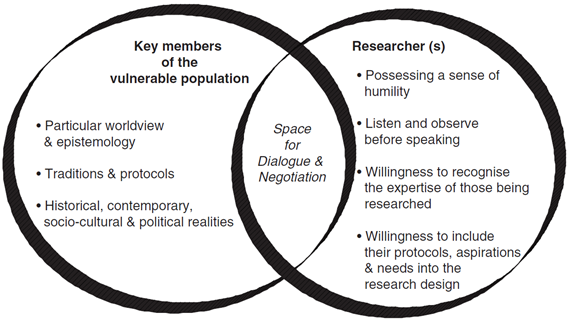
\includegraphics[width=.49\textwidth]{dialogue}
\caption{Creating the space for dialogue and negotiation}
\label{dialoguevulnerable}
\end{figure}
\begin{figure}[H]
\centering
\includegraphics[width=.49\textwidth]{power}
\caption{Power in Research with Vulnerable Populations}
\label{powervulnerable}
\end{figure}

\end{multicols}

Activity: Prisoners w/ mental illness - Perception of Authority
"Authority" - Remove CO's if possible
\begin{itemize}
\item Consent/Assent from guardian/CO/Wardens
\item Needs assessment: Medication, resource 
\item Compensation? 
\item create space to speak to prisoner alone if possible
\item remove identifiers from research if possible to avoid negative consequences for the participant
\item have a plan for crisis 
\item have a plan for lack of medicine or being forced to take medicine
\item have a plan for signs of retaliation from CO's and peers
\end{itemize}

\end{document}
